\documentclass[12pt,a4paper]{report}

% Packages for formatting and functionality
\usepackage[utf8]{inputenc}
\usepackage{geometry}
\geometry{top=1in, bottom=1in, left=1in, right=1in}
\usepackage{graphicx}
\usepackage{listings}
\usepackage{xcolor}
\usepackage{tikz}
\usetikzlibrary{shapes,arrows,positioning,fit,calc,shadows}
\usepackage{hyperref}
\usepackage{titlesec}
\usepackage{caption}
\usepackage{float}

% Hyperlink configuration
\hypersetup{
    colorlinks=true,
    linkcolor=black,
    filecolor=magenta,      
    urlcolor=blue,
    pdftitle={Online Food Delivery System Report},
    pdfpagemode=FullScreen,
}

% Code listing configuration
\definecolor{codegreen}{rgb}{0,0.6,0}
\definecolor{codegray}{rgb}{0.5,0.5,0.5}
\definecolor{codepurple}{rgb}{0.58,0,0.82}
\definecolor{backcolour}{rgb}{0.95,0.95,0.92}

\lstdefinestyle{javastyle}{
    backgroundcolor=\color{backcolour},   
    commentstyle=\color{codegreen},
    keywordstyle=\color{magenta},
    numberstyle=\tiny\color{codegray},
    stringstyle=\color{codepurple},
    basicstyle=\ttfamily\footnotesize,
    breakatwhitespace=false,         
    breaklines=true,                 
    captionpos=b,                    
    keepspaces=true,                 
    numbers=left,                    
    numbersep=5pt,                  
    showspaces=false,                
    showstringspaces=false,
    showtabs=false,                  
    tabsize=4
}

\lstset{style=javastyle}

% Title Page Information
\title{\textbf{Online Food Delivery Order Processing System}\\ \large Implementation & Architecture Report}
\author{Senior Software Architect}
\date{\today}

\begin{document}
%---------------- Cover Page ----------------%
\begin{titlepage}
    \centering
    \vspace*{2cm}
    {\Huge \bfseries Design Patterns \par}
    {\Huge \bfseries Quiz-2 (Assignment) \par}
    
    \vspace{2cm}
    {\Large Name: Ahnaf Shahriar Pias \par}
    \vspace{0.5cm}
    {\Large Student ID: 220042146 \par}
    \vspace{0.5cm}
    {\Large Course Name: Design Patterns  \par}
    \vspace{0.5cm}
    {\Large Course Code: SWE-4501 \par}
    \vspace{0.5cm}
    {\Large Date: January 3 , 2026 \par}
    \vfill
    {\large Department of CSE, IUT \par}
\end{titlepage}

\newpage


% Table of Contents
\tableofcontents
\thispagestyle{empty}
\clearpage

% -------------------------------------------------------------------
% Chapter 1: Introduction
% -------------------------------------------------------------------
\chapter{Introduction}
\pagenumbering{arabic} % Start page numbering here

\section{Project Overview}
The \textbf{Online Food Delivery Order Processing System} is a robust, console-based Java application designed to demonstrate the practical application of advanced software design patterns. The system simulates the lifecycle of a food order—from creation and customization to processing and delivery fee calculation.

The primary objective of this project is to create a cleanly modularized, extensible, and maintainable codebase that adheres to the \textbf{SOLID principles} of object-oriented design. By decoupling core components, the system allows for easy addition of new order types, delivery strategies, and order add-ons without modifying existing code.

\section{Technical Context and Relevance}
In modern software engineering, managing complexity is paramount. As systems grow, hard-coded logic and tight coupling can lead to "spaghetti code" that is difficult to test and maintain. This project addresses these challenges by employing four industry-standard Gang of Four (GoF) design patterns:
\begin{itemize}
    \item \textbf{Factory Pattern}: For decoupling object creation logic.
    \item \textbf{Template Method Pattern}: For enforcing a consistent processing workflow.
    \item \textbf{Strategy Pattern}: For enabling interchangeable algorithms (delivery fees).
    \item \textbf{Decorator Pattern}: For dynamically extending object functionality (add-ons).
\end{itemize}

The implementation serves as a reference architecture for building flexible order processing systems in enterprise environments.

\clearpage

% -------------------------------------------------------------------
% Chapter 2: Implementation Details
% -------------------------------------------------------------------
\chapter{Implementation Details}

This chapter provides an in-depth analysis of the four design patterns employed in the system. It details their individual implementations, their interconnections, and how the client code orchestrates them to achieve a flexible order processing workflow.

\section{Factory Pattern (Order Creation)}
The Factory Pattern is utilized to abstract the object instantiation process. By centralizing the creation logic within the \texttt{OrderFactory}, the system decouples the client code from the concrete classes (\texttt{FastFoodOrder}, \texttt{FineDiningOrder}, etc.).

\subsection{Implementation Logic}
The factory uses a simple static method that takes a string identifier (e.g., "fastfood") and returns the corresponding \texttt{Order} implementation. This adheres to the \textit{Simple Factory} idiom, allowing for easy expansion. If a new order type is introduced, only the factory's switch statement needs modification, keeping the client code untouched.

\begin{lstlisting}[language=Java, caption=OrderFactory: Centralized Object Creation]
public class OrderFactory {
    /**
     * Creates an Order instance based on the provided type.
     * @param orderType The identifier for the order type.
     * @return A concrete implementation of Order.
     */
    public static Order createOrder(String orderType) {
        if (orderType == null) return null;
        switch (orderType.toLowerCase()) {
            case "fastfood": 
                return new FastFoodOrder();
            case "finedining": 
                return new FineDiningOrder();
            case "cloudkitchen": 
                return new CloudKitchenOrder();
            default: 
                throw new IllegalArgumentException("Unknown order type: " + orderType);
        }
    }
}
\end{lstlisting}

\section{Template Method Pattern (Order Processing)}
The Template Method Pattern is pivotal for enforcing a standard operating procedure across all order types. It defines the invariant steps of the order lifecycle while allowing subclasses to provide specific implementations for variant steps.

\subsection{Workflow Definition}
The \texttt{OrderProcessTemplate} abstract class implements the \texttt{Order} interface. It defines a \texttt{final} method \texttt{processOrder()}, which dictates the sequence of operations:
\begin{enumerate}
    \item \texttt{validateOrder()}: Common implementation for all orders.
    \item \texttt{prepareFood()}: Abstract method, must be implemented by subclasses.
    \item \texttt{packageOrder()}: Common implementation.
    \item \texttt{dispatchOrder()}: Common implementation.
\end{enumerate}

\begin{lstlisting}[language=Java, caption=OrderProcessTemplate: Enforcing the Algorithm Skeleton]
public abstract class OrderProcessTemplate implements Order {
    
    // The Template Method - Final to prevent overriding the workflow
    @Override
    public final void processOrder() {
        System.out.println("\n--- Processing Order ---");
        validateOrder();
        prepareFood(); // The primitive operation that varies
        packageOrder();
        dispatchOrder();
    }
    
    // Abstract step to be implemented by concrete classes
    protected abstract void prepareFood();
    
    protected void validateOrder() { 
        System.out.println("Step 1: Validating order details..."); 
    }
    
    protected void packageOrder() {
        System.out.println("Step 3: Packaging food safely...");
    }
    
    protected void dispatchOrder() {
        System.out.println("Step 4: Dispatching delivery partner...");
    }
}
\end{lstlisting}

\subsection{Concrete Implementation Example}
A concrete class, such as \texttt{FastFoodOrder}, only needs to focus on its specific preparation logic.

\begin{lstlisting}[language=Java, caption=FastFoodOrder: Specific Step Implementation]
public class FastFoodOrder extends OrderProcessTemplate {
    @Override
    protected void prepareFood() {
        System.out.println("Step 2: Assembling burger and frying fries...");
    }
    
    // Also implements getDescription() and getCost() from Order interface
}
\end{lstlisting}

\section{Strategy Pattern (Delivery Fee Calculation)}
The Strategy Pattern is employed to handle the volatile logic of delivery fee calculations. Instead of embedding fee logic within the order classes (which would violate the Single Responsibility Principle), the calculation is delegated to interchangeable strategy objects.

\subsection{Decoupling Algorithm from Context}
The \texttt{DeliveryFeeStrategy} interface acts as the abstraction. Concrete strategies implement specific pricing rules.

\begin{lstlisting}[language=Java, caption=DeliveryFeeStrategy Interface and Implementation]
public interface DeliveryFeeStrategy {
    double calculateFee(Order order);
}

// Concrete Strategy: Surge Pricing
public class SurgeDeliveryStrategy implements DeliveryFeeStrategy {
    @Override
    public double calculateFee(Order order) {
        // High base fee + 10% of order cost
        return 15.0 + (order.getCost() * 0.10);
    }
}
\end{lstlisting}

\section{Decorator Pattern (Dynamic Add-ons)}
The Decorator Pattern addresses the requirement for optional, stackable order enhancements (like "Gift Wrap" or "Priority Handling") without creating a combinatorial explosion of subclasses.

\subsection{Recursive Composition}
The \texttt{OrderDecorator} abstract class implements the \texttt{Order} interface and contains a reference to an \texttt{Order} object. This allows decorators to wrap other decorators or concrete orders, building a chain of responsibility where each layer adds its own cost and description.

\begin{lstlisting}[language=Java, caption=OrderDecorator and Concrete Decorator]
public abstract class OrderDecorator implements Order {
    protected Order decoratedOrder;

    public OrderDecorator(Order decoratedOrder) {
        this.decoratedOrder = decoratedOrder;
    }

    @Override
    public void processOrder() {
        decoratedOrder.processOrder(); // Delegation
    }
}

public class GiftWrapDecorator extends OrderDecorator {
    public GiftWrapDecorator(Order decoratedOrder) {
        super(decoratedOrder);
    }

    @Override
    public String getDescription() {
        return decoratedOrder.getDescription() + " + Gift Wrap";
    }

    @Override
    public double getCost() {
        return decoratedOrder.getCost() + 5.0; // Additive cost
    }
}
\end{lstlisting}

\section{Pattern Integration and Client Usage}
The true power of this architecture lies in how these patterns interact. The client code (\texttt{Main.java}) orchestrates the flow:
\begin{enumerate}
    \item \textbf{Creation}: The \textbf{Factory} creates the base order object.
    \item \textbf{Extension}: The \textbf{Decorator} wraps the order object to add features.
    \item \textbf{Processing}: The \textbf{Template Method} executes the workflow on the (potentially decorated) order.
    \item \textbf{Calculation}: The \textbf{Strategy} calculates the fee based on the final state of the order.
\end{enumerate}

\begin{lstlisting}[language=Java, caption=Client Code Integration (Main.java)]
// 1. Creation via Factory
Order order = OrderFactory.createOrder("finedining");

// 2. Dynamic Extension via Decorators (Stacking)
order = new GiftWrapDecorator(order);
order = new PriorityHandlingDecorator(order);

// 3. Strategy Selection
DeliveryFeeStrategy strategy = new SurgeDeliveryStrategy();

// 4. Execution
// Template Method runs the workflow
order.processOrder(); 

// Strategy calculates fee using the decorated order's total cost
double fee = strategy.calculateFee(order);
\end{lstlisting}

This approach ensures that the "Processing" logic is isolated from the "Creation" logic, and the "Cost Calculation" is independent of the "Order Structure".

\clearpage

% -------------------------------------------------------------------
% Chapter 3: System Architecture
% -------------------------------------------------------------------
\chapter{System Architecture}

The system architecture is visualized below using a comprehensive UML Class Diagram. This diagram illustrates the structural relationships between the components, highlighting the implementation of the four design patterns.

\vspace{0.5cm}

\begin{figure}[H]
\centering
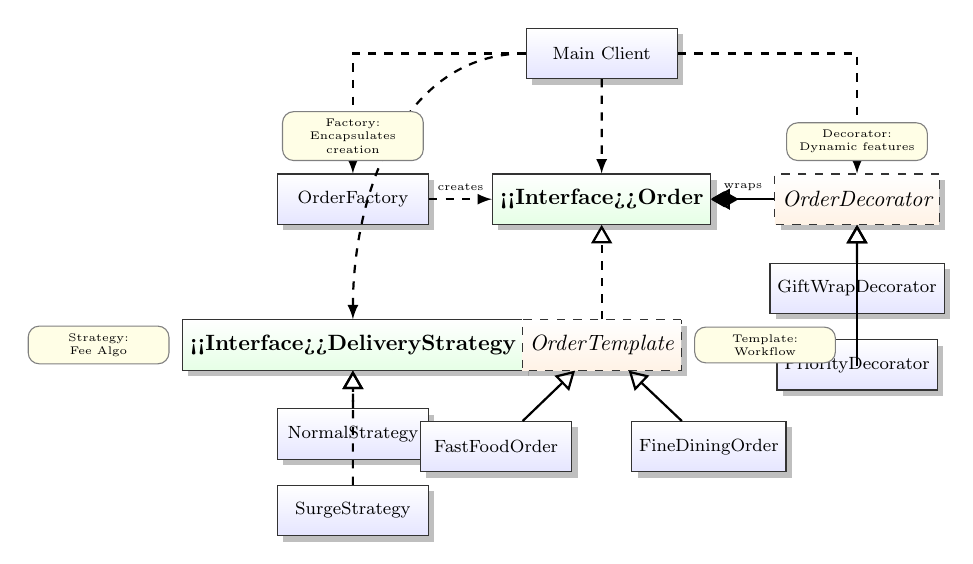
\begin{tikzpicture}[
    scale=0.8,
    transform shape,
    font=\footnotesize,
    node distance=1.2cm and 0.5cm,
    % Styles
    interface/.style={
        rectangle, 
        draw=black!80, 
        top color=white, bottom color=green!10, 
        text centered, 
        minimum height=0.8cm, 
        minimum width=2.4cm,
        drop shadow,
        font=\bfseries
    },
    abstract/.style={
        rectangle, 
        draw=black!80, 
        top color=white, bottom color=orange!10, 
        text centered, 
        minimum height=0.8cm, 
        minimum width=2.4cm,
        dashed,
        drop shadow,
        font=\itshape
    },
    class/.style={
        rectangle, 
        draw=black!80, 
        top color=white, bottom color=blue!10, 
        text centered, 
        minimum height=0.8cm, 
        minimum width=2.4cm,
        drop shadow
    },
    note/.style={
        rectangle, 
        draw=gray, 
        fill=yellow!10, 
        text width=2.0cm, 
        font=\tiny, 
        rounded corners,
        align=center
    },
    % Line Styles
    inherit/.style={draw, -open triangle 60, thick},
    realize/.style={draw, dashed, -open triangle 60, thick},
    decorate/.style={draw, -diamond, thick},
    depend/.style={draw, dashed, -latex, thick},
    assoc/.style={draw, -latex, thick}
]

% --- Nodes ---

% Center Hub: Order Interface
\node[interface] (Order) {<<Interface>>\\Order};

% Left Column: Factory & Strategy
\node[class, left=1.0cm of Order] (Factory) {OrderFactory};
\node[interface, below=1.5cm of Factory] (Strategy) {<<Interface>>\\DeliveryStrategy};
\node[class, below=0.6cm of Strategy] (NormalStrategy) {NormalStrategy};
\node[class, below=0.4cm of NormalStrategy] (SurgeStrategy) {SurgeStrategy};

% Right Column: Decorator
\node[abstract, right=1.0cm of Order] (Decorator) {OrderDecorator};
\node[class, below=0.6cm of Decorator] (GiftWrap) {GiftWrapDecorator};
\node[class, below=0.4cm of GiftWrap] (Priority) {PriorityDecorator};

% Center Column (Bottom): Template Method
\node[abstract, below=1.5cm of Order] (Template) {OrderTemplate};
\node[class, below left=0.8cm and -0.8cm of Template] (FastFood) {FastFoodOrder};
\node[class, below right=0.8cm and -0.8cm of Template] (FineDining) {FineDiningOrder};

% Top: Main Client
\node[class, above=1.5cm of Order, fill=gray!20] (Main) {Main Client};

% --- Relationships ---

% 1. Factory
\draw[depend] (Factory) -- node[above, font=\tiny] {creates} (Order);

% 2. Decorator
\draw[realize] (Decorator) -- (Order);
\draw[inherit] (GiftWrap) -- (Decorator);
\draw[inherit] (Priority) -| (Decorator);
\draw[decorate] (Decorator) -- node[above, font=\tiny] {wraps} (Order);

% 3. Template
\draw[realize] (Template) -- (Order);
\draw[inherit] (FastFood) -- (Template);
\draw[inherit] (FineDining) -- (Template);

% 4. Strategy
\draw[realize] (NormalStrategy) -- (Strategy);
\draw[realize] (SurgeStrategy) -- (Strategy);

% 5. Main Interactions
\draw[depend] (Main) -| (Factory);
\draw[depend] (Main) -- (Order);
\draw[depend] (Main) -| (Decorator);
\draw[depend] (Main) to[out=180,in=90] (Strategy);

% --- Annotations ---
\node[note, above=0.2cm of Factory] {Factory:\\Encapsulates creation};
\node[note, above=0.2cm of Decorator] {Decorator:\\Dynamic features};
\node[note, left=0.2cm of Strategy] {Strategy:\\Fee Algo};
\node[note, right=0.2cm of Template] {Template:\\Workflow};

\end{tikzpicture}
\caption{Architectural Class Diagram}
\label{fig:uml_improved}
\end{figure}

\section{Diagram Legend}
\begin{itemize}
    \item \textbf{Green Box}: Interface
    \item \textbf{Orange Box (Dashed)}: Abstract Class
    \item \textbf{Blue Box}: Concrete Class
    \item \textbf{Solid Line with Triangle}: Inheritance (extends)
    \item \textbf{Dashed Line with Triangle}: Realization (implements)
    \item \textbf{Line with Diamond}: Aggregation (Decorator holds Order)
    \item \textbf{Dashed Arrow}: Dependency
\end{itemize}

\clearpage


% -------------------------------------------------------------------
% Chapter 5: Conclusion
% -------------------------------------------------------------------
\chapter{Conclusion}

\section{Lessons Learned}
Implementing this system reinforced the importance of the \textbf{Dependency Inversion Principle}. By coding to interfaces (\texttt{Order}, \texttt{DeliveryFeeStrategy}) rather than concrete implementations, the system became significantly easier to extend. The combination of the Template Method and Decorator patterns demonstrated how inheritance and composition can work together to solve different aspects of the same problem (workflow structure vs. dynamic capabilities).

\section{Potential Improvements}
While the current implementation fulfills the architectural requirements, future enhancements could include:
\begin{itemize}
    \item \textbf{Database Integration}: Persistence of orders using JPA/Hibernate.
    \item \textbf{Concurrency}: Processing multiple orders simultaneously using Java Threads.
    \item \textbf{Configuration Injection}: Using a framework like Spring to inject specific strategies via configuration files rather than hard-coding them in `Main`.
\end{itemize}

\section{Final Remarks}
The Online Food Delivery Order Processing System successfully demonstrates that applying design patterns results in code that is readable, modular, and resilient to change. The architecture allows business rules (like pricing strategies) to evolve independently of the core domain objects, satisfying the goals of modern software design.

\end{document}
